\usetikzlibrary{calc, arrows.meta, intersections, patterns, positioning, shapes.misc, fadings, through,decorations.pathreplacing}

\begin{figure}[t]
\centering
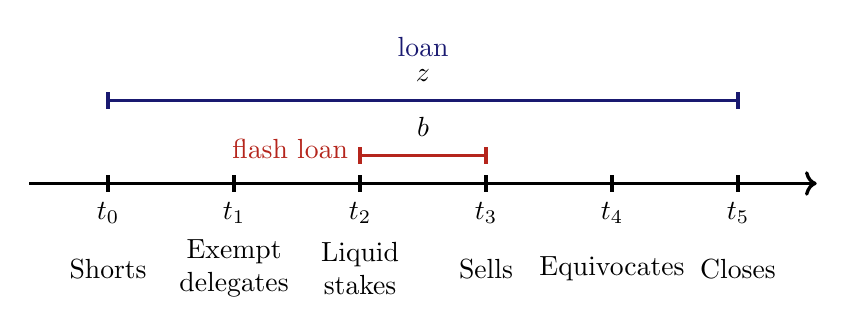
\begin{tikzpicture}[very thick, black]

\coordinate (distance) at (1.6,0);

\coordinate (O) at (-1,0); % Origin
\coordinate (P0) at (0, 0);
\coordinate (P1) at ($(P0) + (distance)$);
\coordinate (P2) at ($(P1) + (distance)$);
\coordinate (P3) at ($(P2) + (distance)$);
\coordinate (P4) at ($(P3) + (distance)$);
\coordinate (P5) at ($(P4) + (distance)$);
\coordinate (F) at (9,0); %End


%% Timeline
\draw[->] (O) -- (F);


%% Ticks
\foreach \x in {P0,P1,P2,P3,P4,P5}
\draw ($(\x) - (0,3pt)$) -- ($(\x) + (0,3pt)$);


%% t_0
\draw (P0) node[below=3pt](T0) {$t_0$} ;
\node[yshift=-20pt] at (T0) {%
	Shorts};

%% t_1
\draw (P1) node[below=3pt](T1) {$t_1$} ;
\node[align=center,yshift=-20pt] at (T1) {%
	Exempt\\delegates};

%% t_2
\draw (P2) node[below=3pt](T2) {$t_2$} ;
\node[yshift=-20pt,align=center] at (T2) {%
	Liquid\\stakes};

%% t_3
\draw (P3) node[below=3pt](T3) {$t_3$} ;
\node[yshift=-20pt] at (T3) {%
	Sells};

%% t_4
\draw (P4) node[below=3pt](T4) {$t_4$} ;
\node[yshift=-20pt] at (T4) {%
  Equivocates};

%% t_5
\draw (P5) node[below=3pt](T5) {$t_5$} ;
\node[yshift=-20pt] at (T5) {%
  Closes};


%% Loans
\coordinate[above=10pt] (R1) at (P2);
\coordinate[above=10pt] (R2) at (P3);
\coordinate[above=30pt] (R3) at (P0);
\coordinate[above=30pt] (R5) at (P5);


\draw[color=BrickRed] ($(R1) + (0,3pt)$) -- ($(R1) + (0,-3pt)$);
\draw[color=BrickRed] ($(R2) + (0,3pt)$) -- ($(R2) + (0,-3pt)$);
\draw[color=BrickRed] (R1) -- (R2) node[color=black,midway, above=3pt](L1) {$b$ {\tiny \asset}};

\node[text=BrickRed,xshift=-48pt,yshift=-8pt] at (L1) {flash loan};

\draw[color=MidnightBlue] ($(R3) + (0,3pt)$) -- ($(R3) + (0,-3pt)$);
\draw[color=MidnightBlue] ($(R5) + (0,3pt)$) -- ($(R5) + (0,-3pt)$);
\draw[color=MidnightBlue] (R3) -- (R5) node[color=black,midway, above=3pt](L2) {$z$ {\tiny \stasset}};
\node[text=MidnightBlue,above=3pt] at (L2) {loan};
\end{tikzpicture}

\caption{Timeline of the exempt delegation attack.}
\label{fig:exempt-timeline}
\end{figure}
